%!TEX root = main.tex

\section{Introduction}


%A desirable video streaming protocol should maximize user-perceived video quality under dynamic network conditions.
A fundamental tension in any video streaming protocol is between the encoding efficiency and the agility of adaptation.
If we know that a video segment will be streamed under a stable throughput, we can maximize the quality (\eg high resolution, no rebuffering) by aggressively eliminating the pixel-level spatio-temporal redundancies.
But if a video is encoded too aggressively, it would be hard to adapt the quality level fast enough to cope with bandwidth fluctuations.
%A case-in-point of this tradeoff is DASH~\cite{??,??,??}, which recently took hold as the mainstream video protocol. 
%It balances the encoding efficiency and adaptation by splitting the video to fixed-length chunks (4-10 seconds) each encoded in discrete quality levels, allowing it to switch quality at chunk boundaries.


The recent surge of \vr videos poses new challenges to this tension between encoding efficiency and adaptation agility. 
As many major content providers roll out \vr videos~\cite{??,??,??,??,??}, 
it is clear that streaming \vr videos is more challenging than streaming traditional videos for two reasons.
First, \vr videos must stream much more data (both in \vr and in higher resolution) without any interruption in order to create the immersive experience.
Second, although one can use less bandwidth by streaming only the region directly facing the viewer (around \fillme\% of the panoramic view), doing so will force the encoder to use chunks of shorter durations (typically, one second) to keep up with the viewport movement, which reduces the encoding efficiency.


In this paper, we argue that there are still many unexploited opportunities to improve \vr video quality, through a {\em deeper understanding of how viewers perceive the \vr video quality}.
The assumption behind many existing \vr video protocols is that the perceived quality of a region depends only on how far the region is to the viewport center.
However, we found that the perceived quality of a \vr video can be heavily influenced by several other factors---the {\em velocity} of the head movement, the {\em relative depth} of the viewed objects, and the {\em relative brightness} of the objects compared to those the user have just watched. 
%That is the viewport position and video quality, we found that a \vr video at least three reasons: the velocity of head movement, how the relative depth of the viewed objects, as well as the brightness of the objects compared to those the user have just watched. 

In our user study, for instance, when shown the same video at different quality levels, most viewers can perceive quality difference between videos when their viewport is static, but cannot tell any visible difference when the users move their viewport (\eg shaking head or browsing the landscape).
Similarly, how sensitive the viewer is to a given quality difference depends greatly on how further/closer the object is or how much brighter/darker compared to objects that the viewer just saw.
Note that unlike in traditional videos, these factors are driven by ``user behaviors'' unique to \vr videos (see \S\ref{sec:motivation} for more discussions).




The findings that humans have only bounded sensitivity to quality degradation can have great implications for \vr video streaming. 
In theory, an ideal video streaming protocol can maximize perceived quality, if it always increases quality by a perceivable amount and saves bandwidth by lowering the quality by just an imperceivable amount. 
Based on our user study over \fillme videos and \fillme viewers, we found that one can save \fillme\% bandwidth without any drop in perceived quality! (More discussions in \S\ref{sec:motivation:potential})



\begin{figure}[t!]
  \centering
  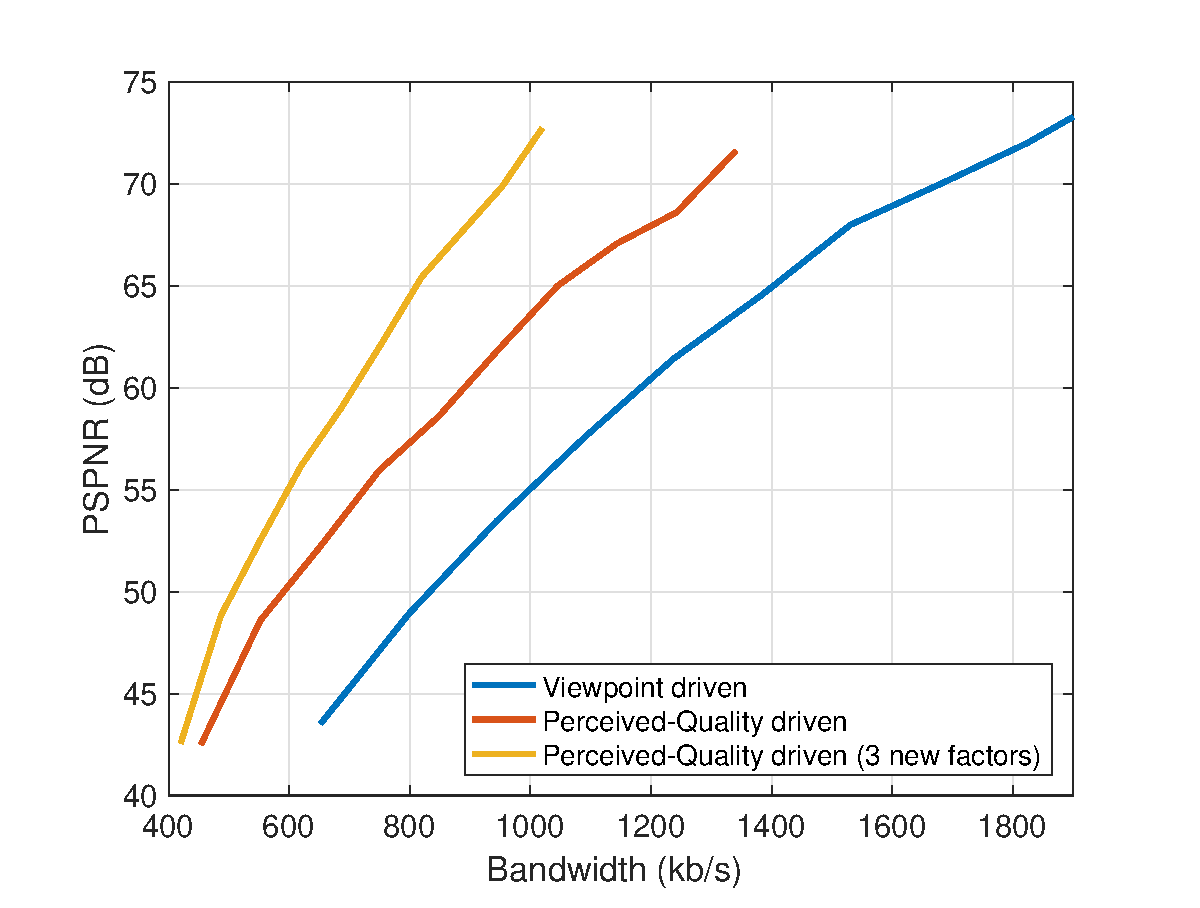
\includegraphics[width=2.5in]{images/improvement.eps}
  \caption{Effectiveness of \name at reducing the bandwidth consumption and improving QoE. \jc{TODO. an example graph with two curves comparing \name and a canonical \vr video streaming protocol. }}
  \label{fig:intro-improvement}
  \end{figure}

The root of these opportunities is the fact that people have a limited span of attention.
Consider when a viewer moves her head quickly, it does increase the viewport-covered area that has to be streamed and rendered, but the viewer's attention per-pixel (\ie sensitivity to quality degradation) actually drops due to the limited span of attention.
Similar ideas have been used by video encoders to compress videos via exploiting the ``Just Noticeable Difference'' (JND)~\cite{??,??,??}---the minimal visual difference perceivable by humans, \eg viewers generally have larger JND when watching a more complex scene. 
However, conventional JND only models the content-specific factors (since it assumes a static viewport), as opposed to the factors driven by changes . 

This paper presents {\em \name}, an encoding and streaming system that optimizes the user-perceived quality of \vr videos. 
\name makes three contributions.

\vspace{0.2cm}
{\em First, \name is based on a new unifying JND model which incorporates the factors driven by \vr video viewer actions.}
We did a user study to model the impact of four viewer action-driven factors---movement velocity, relative depth-of-view, relative darkness, and distance-to-viewport---on viewer's sensitivity to quality degradation.
The resulting JND model, referred to as {\em \vrjnd}, can predict, for any given video and viewport trajectory, the amount of quality changes  that are likely be perceivable by the viewer.

An interesting empirical finding is that the new viewer-driven factors are largely independent to each other.
This vastly simplifies the modeling of impact of multiple factors on JND, which would otherwise have to explore the space of a exponential number of combinations of multiple factors.
Their likely independence might explained by \jc{what's the intuition here?}


\vspace{0.2cm}
{\em Second, \name is based on a novel chunking mechanism to fully utilize the new JND model.}
To best utilize the proposed \vrjnd,  a video should ideally be segmented spatially into tiles whose boundaries are aligned with those of the values in the \vrjnd, which typically are the boundaries of objects.
Unfortunately, we found the existing equal-sized square tiling (\eg 12$\times$6) often is far from ideal---the tiles can be too coarse- or too fine-grained. 
In fairness, the square tiling is designed to serve only one purpose of differentiating regions closer to the viewport center from the rest.

\name takes a different path. 
\name splits the \vr video into square tiles of different sizes, each of which is one-second in duration and roughly matches the objects in the video. Each tile is then encoded in multiple levels of quantization parameter (QPs), like in existing tiling schemes.
In some sense, this is a compromise between the more radical region-of-interest encoding (in which each object can be encoded differently) and the square tiling which simplifies the rendering of multiple tiles each with different QP levels.



\vspace{0.2cm}
{\em Finally, \name uses a DASH-compatible streaming protocol that adapts to dynamic user actions and network conditions.}
A key challenge of \vrjnd is that any \vrjnd-based quality adaptation needs the access to the video data on the server (\ie cannot be done by the client itself), so it is incompatible with the mainstream DASH protocols which stream videos from stateless HTTP web servers. 
%to determine the perceived quality of a chunk require some computation based on the video data on the server side, so in theory, it is incompatible with the mainstream DASH protocols which stream videos from stateless HTTP web servers.
This is not a problem in non-\vr videos or existing \vr video protocols, because calculating the perceived quality of a chunk only depends on the available bandwidth and user viewport, both are locally accessible on the client side.
However, the perceived quality in \vrjnd depends on the video content and user actions (\ie viewport trajectory and its projection), so the client cannot estimate the user-perceived quality without having the video content in the first place. 
%One approach to this conundrum is to let the video client upload the user action information to the server which then makes adaptation decisions, but this goes against DASH's HTTP-based architecture.

Instead, in this work, we have taken a pragmatic stance to work within the constraints that have spurred the growth of video traffic---streaming videos from web servers over HTTP, like in DASH.
The basic idea is that it is possible to pre-compute the best quality levels for only a few carefully picked possible values of the user action information (viewport trajectory and its projection), and send these estimates as part of the DASH metafile to the client at the beginning of a video session. 
Thus, during playtime the client will be able to estimate the quality level by finding a ``nearest neighbor'' in the user inputs that have been pre-computed. 
The intuition behind pre-computing only a few user-action inputs is an empirical observation that in \vrjnd the impact of the user-action input is non-linear; \eg when the viewport movement speed is over some threshold, its impact on \vrjnd and the QP adaptation changes only marginally (probably because the viewer will be very insensitive).


\vspace{0.2cm}
We implemented a prototype of \name.
\jc{on what platform}
We ran a pilot study on one content provider with \fillme sessions. \jc{how many viewers? what types of videos?}

Our experiments show that \name can save 45\% bandwidth compared with state-of-art 360-video streaming solutions, without decrease of perceived quality.
\jc{add a line to describe the final user-rating based end-to-end experiments}

